%!TeX program = lualatex
\renewcommand{\thelektion}{L09 \textperiodcentered{} Logische Gatter II}
\usetikzlibrary{circuits.logic.US}

\begin{frame}\lessontitle{Lektion 09}{Logische Gatter II}{NAND, funktionale Vollständigkeit und der Halbaddierer \textperiodcentered{} Skript, Kapitel 4}\end{frame}

\begin{frame}\FDUtitle{Rückblick}
\begin{center}
Letztes Mal: NOT, AND, OR -- die drei elementaren Booleschen Verknüpfungen.
\vspace{4mm}

Heute: ein einziges Gatter, aus dem sich \textbf{alle} anderen bauen lassen.
\end{center}
\end{frame}

\begin{frame}\FDUtitle{Das NAND-Gatter}
\begin{columns}[c,onlytextwidth]
\begin{column}{.46\textwidth}
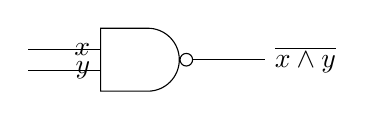
\begin{tikzpicture}[circuit logic US, scale=1.3]
  \node[nand gate, draw] (nand1) {};
  \draw (nand1.input 1) ++(-0.7,0) -- (nand1.input 1) node[left] {$x$};
  \draw (nand1.input 2) ++(-0.7,0) -- (nand1.input 2) node[left] {$y$};
  \draw (nand1.output) -- ++(0.7,0) node[right] {$\overline{x \wedge y}$};
\end{tikzpicture}
\end{column}
\begin{column}{.46\textwidth}
\begin{tabular}{c|c||c}
    $x$ & $y$ & $\overline{x \wedge y}$ \\\midrule\midrule
    0 & 0 & 1 \\\midrule
    0 & 1 & 1 \\\midrule
    1 & 0 & 1 \\\midrule
    1 & 1 & 0 \\
\end{tabular}
\end{column}
\end{columns}
\vspace{3mm}
\begin{center}$x \uparrow y = \overline{x \wedge y}$ -- die Negation von AND.\end{center}
\end{frame}

\begin{frame}\FDUtitle{Funktional vollständig}
\begin{center}
Aus Kombinationen von NAND-Gattern lassen sich \textbf{alle} anderen logischen Funktionen nachbauen.
\vspace{4mm}

\textbf{Übung}: Stellen Sie die Wahrheitstabelle von $x \uparrow x$ auf. Was fällt auf?
\end{center}
\only<2->{
\begin{center}
\begin{tabular}{c||c|c}
    $x$ & $x \wedge x$ & $\overline{x \wedge x}$ \\\midrule\midrule
    0 & 0 & 1 \\\midrule
    1 & 1 & 0 \\
\end{tabular}
\end{center}
\begin{center}\color{FDUteal}\bfseries $x \uparrow x = \overline{x}$ -- ein NOT-Gatter aus einem einzigen NAND!\end{center}
}
\end{frame}

\begin{frame}\FDUtitle{Warum ist das praktisch relevant?}
\begin{center}
In vielen Fertigungsprozessen ist es technologisch günstig, sehr grosse Schaltungen aus nur \textbf{einem} standardisierten Gattertyp aufzubauen -- NAND ist ein solcher \enquote{Universalbaustein}.
\end{center}
\end{frame}

{\setbeamertemplate{footline}{\darkfootline}
\begin{frame}\sectionframe[FDUgreen]{Der Halbaddierer}{Wenn Gatter tatsächlich rechnen}
\end{frame}}

\begin{frame}\FDUtitle{Zwei Bits addieren}
\begin{center}
\begin{tabular}{cc}
    $x$ & $y$ \\\midrule
    0 & 0 \\
    0 & 1 \\
    1 & 0 \\
    1 & 1 \\
\end{tabular}
\quad$\longrightarrow$\quad
\begin{tabular}{cc}
    Übertrag $c$ & Summe $s$ \\\midrule
    0 & 0 \\
    0 & 1 \\
    0 & 1 \\
    1 & 0 \\
\end{tabular}
\end{center}
\begin{center}
Erkennen Sie zwei bekannte Gatter in diesen Spalten?
\end{center}
\only<2->{\begin{center}\color{FDUteal}\bfseries $s = x \oplus y$ (XOR), \quad $c = x \wedge y$ (AND)\end{center}}
\end{frame}

\begin{frame}\FDUtitle{Schaltplan des Halbaddierers}
\begin{center}
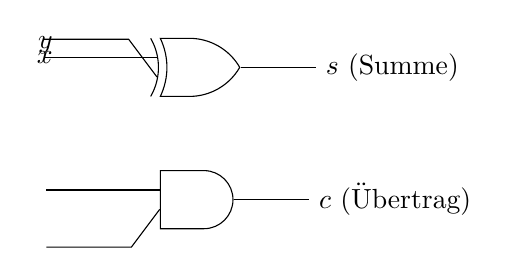
\begin{tikzpicture}[circuit logic US, scale=1.2]
    \node[xor gate, draw] (xor1) at (2,0.5) {};
    \node[and gate, draw] (and1) at (2,-0.9) {};
    \draw (xor1.input 1) ++(-1.2,0) -- ++(0.5,0) -- (xor1.input 1) node[left,xshift=-1.2cm] {$x$};
    \draw (and1.input 1) ++(-1.2,0) -- ++(0.5,0) -- (and1.input 1);
    \draw (xor1.input 2) ++(-1.2,0.4) -- ++(0.9,0) -- (xor1.input 2) node[left,xshift=-1.2cm,yshift=0.4cm] {$y$};
    \draw (and1.input 2) ++(-1.2,-0.4) -- ++(0.9,0) -- (and1.input 2);
    \draw (xor1.output) -- ++(0.8,0) node[right] {$s$ (Summe)};
    \draw (and1.output) -- ++(0.8,0) node[right] {$c$ (Übertrag)};
\end{tikzpicture}
\end{center}
\begin{center}XOR liefert die Summe, AND den Übertrag.\end{center}
\end{frame}

\begin{frame}\FDUtitle{Übung: Halbaddierer-Wahrheitstabelle}
\begin{center}
\small
\begin{tabular}{c|c||c|c|c|c}
    $x$ & $y$ & Summe $s$ ($x \oplus y$) & Übertrag $c$ ($x \land y$) & Binär $(cs)_2$ & Dezimal \\\midrule\midrule
    0 & 0 & \only<2->{0} & \only<2->{0} & \only<2->{$00_2$} & \only<2->{0} \\\midrule
    0 & 1 & \only<2->{1} & \only<2->{0} & \only<2->{$01_2$} & \only<2->{1} \\\midrule
    1 & 0 & \only<2->{1} & \only<2->{0} & \only<2->{$01_2$} & \only<2->{1} \\\midrule
    1 & 1 & \only<2->{0} & \only<2->{1} & \only<2->{$10_2$} & \only<2->{2} \\
\end{tabular}
\end{center}
\only<2->{\begin{center}\color{FDUteal}\bfseries Der Halbaddierer berechnet alle 4 Fälle der 1-Bit-Addition exakt korrekt!\end{center}}
\end{frame}

\auftragframe{Kapitel 4, Abschnitte \enquote{Das NAND-Gatter} und \enquote{Kombinierte Schaltungen: der Halbaddierer}}{%
\aufgabebox{NOT aus NAND konstruieren}\\[3mm]
\challengebox{Wie liesse sich ein AND-Gatter aus NAND-Gattern bauen?}
}

